\chapter{Použité technologie}
Tato kapitola shrnuje a představuje hlavní technologie využité při řešení a implementaci projektu.

\section{Frontend}
Za frontend je v~souvislosti s~programováním a návrhem aplikace považováno to, co běžně vidí uživatel dané aplikace. Jedná se o~vizuální stránku programu, díky které lze komunikovat s~tzv. backendem (viz dále) – to znamená, že musí jednak správně interagovat s~uživatelem (např. umožnit uživateli si v~e-shopu vybrat zboží, zpracovat další potřebné údaje poskytnuté uživatelem a následně zboží objednat), ale i se serverem (např. posílat validní data a instrukce od uživatele na server).

Lze ji také označit za „klientskou stranu“ aplikace, jelikož je tvořena primárně pro běžnou a intuitivní obsluhu lidmi, kteří nemusí a ani nepotřebují rozumět technologiím, na kterých tato část funguje. \cite{FEvsBE}

	\subsection{Javascript}
	JavaScript je multiplatformní, objektově orientovaný, událostmi řízený skriptovací jazyk, který je používán primárně při tvorbě webových stránek. Je určen především pro tvorbu klientské strany, ale např. díky prostředí Node.js lze v~něm dnes psát i serverovou část aplikace. \cite{JS1}\cite{JS2}
	
	Psát web v~čistém Javascriptu dnes v~souvislosti s~pokročilejšími webovými aplikacemi s~největší pravděpodobností postrádá smysl, jelikož zde existují tzv. javascriptové frameworky, které za nás řeší nejrůznější problémy (jak technické, tak i bezpečnostní), které bychom museli implementovat v~čistém Javascriptu ručně. Tento projekt není výjimkou, a proto byl při tvoření klientské strany použit framework VueJS, který je představen níže.
	
	\subsection{VueJS}
	VueJS je progresivní open-source framework určený k~tvorbě uživatelských rozhraní. Jedná se framework psaný v~jazyce Javascript, ale lze ho psát i v~Typescriptu. Tento framework je vhodný primárně jen pro účely viditelné část aplikace – nelze v~něm např. programovat chování serveru. \cite{VueJS1}
	
	Svou popularitu si získal především tím, že je vyvíjen komunitou, a strukturou kódu, ve kterém je psán (viz obrázek \ref{fig:vue_kod_komponenty}). Kód jednotlivých komponent je tvořen třemi základními částmi:
	
	\begin{itemize}
		\item \textbf{Template}: část určená pro návrh struktury komponenty v~HTML
		\item \textbf{Script}: část určená pro tvoření logiky a manipulaci s~daty v~komponentě v~Javascriptu
		\item \textbf{Style}: část určená pro stylování komponenty v~CSS
	\end{itemize}

	Nutno zmínit, že se jedná o~framework, který je vytvořen právě pro práci s~komponentami – znamená to, že je vhodné jednotlivé části aplikace rozdělovat na jednotlivé komponenty, které lze použít později v~jiném místě aplikace. Tento přístup vede k~udržitelnosti aplikace. \cite{VueJSSyntax}\cite{VueJS2}
	
	\begin{figure}[h]
		\centering
		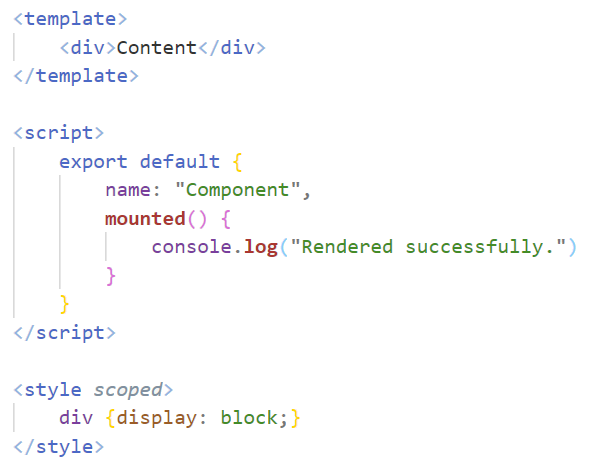
\includegraphics[width=0.8\textwidth]{img/vue_kod_komponenty.png}
		\caption{Ukázka struktury kódu VueJS komponenty}
		\label{fig:vue_kod_komponenty}
	\end{figure}
	
	\subsection{Bootstrap}
	Bootstrap je open-source framework určený především pro stylování běžných komponent webových aplikací. Styly se aplikují na HTML ve formě tříd, kterým jsou interně předepsány parametry, jakým způsobem má být daný element nastylován. Také obsahuje předem hotové styly pro běžné komponenty jako jsou např. formuláře a jejich prvky, navigační lišty, modální okna atp. \cite{Bootstrap1}\cite{Bootstrap2}\cite{Bootstrap3}
	
	\subsection{NPM}\label{sec:npm}
	NPM je rozsáhlý open-source správce balíčků pro Javascript. Je využíván zejména k~přidávání komunitou vytvořených balíčků do vlastních projektů či k~sdílení vlastního balíčku - ty jsou uloženy v~tzv. registru, což je veřejná databáze Javascriptového softwaru. K~instalaci těchto balíčků se nejčastěji používá CLI (Command Line Interface), kterým tento správce disponuje. \cite{NPM}
	
	V~tomto projektu byl využit zejména k~přidání a správě balíčků na frontendové části společně s~VueJS.

\section{Backend}
Termínem backend označujeme část aplikace, která pro běžného uživatele zpravidla není vidět. Jedná se o~administrátorskou část, ve které administrátor konfiguruje, jak se aplikace bude při jednotlivých situacích chovat. Backend, jako samostatná část aplikace, poté slouží ke zpracování dat – např. vyřizuje příchozí požadavky od frontendu nebo na frontend sama zasílá konkrétní data.

Backend může být také zamýšlen jako prostředí pro správu např. obsahu webu. Příkladem může být e-shop, kde na backendu bude moci administrátor např. přidávat jednotlivé zboží nebo spravovat veškeré objednávky.  \cite{BE1}\cite{BE2}
	
	\subsection{PHP}
	PHP (zkr. pro Hypertext Preprocessor) je open-source multiplatformní skriptovací jazyk. Je používán především pro vývoj webových aplikací a může být vložen přímo v~souborech HTML. V~rámci základních informací lze zmínit, že podporuje procedurální i objektově-orientované programování a dokáže pracovat s~velkým množstvím databázových systémů. Oproti Javascriptu je kód spouštěn přímo na serveru, kde generuje HTML, které je předáváno dále na klientskou stranu uživateli. \cite{PHP1}\cite{PHP2}
	
	Hlavním důvodem, proč byl pro tento projekt jazyk PHP vybrán, byla jednoduchost syntaxe jazyka a obecně nižší provozní náklady. V~jazyce PHP je napsán framework Laravel, ve kterém je tvořena backendová část projektu.
	
	\subsection{Laravel}
	Laravel je open-source framework pro tvorbu webových aplikací v~jazyce PHP. Řeší za vývojáře mnoho běžné implementovaných funkcí jako např. autentifikaci, přesměrovávání, správu session a cookies souborů, tvoření databázových migrací nebo testování aplikace. Je inspirován frameworky jako Ruby on Rails, ASP.NET MVC nebo Sinatra a snaží se o~to, aby vývoj webových aplikací byl pro vývojáře co nejpohodlnější a nejintuitivnější. \cite{Laravel1} Framework vychází z~návrhového vzoru MVC \cite{LaravelMVC}.
	
	Dále samotný Laravel disponuje velkým ekosystémem přídavků, funkcí a knihoven, díky kterým si můžeme při vývoji ještě více usnadnit práci. \cite{LaravelEco} V~mém projektu ze zmíněného ekosystému využívám např. Laravel Sanctum pro autentifikaci single-page aplikací.
	
		\subsubsection{Návrhový vzor MVC}
		MVC (zkr. pro Model-View-Controller) je architektonický vzor, jehož základní myšlenkou je oddělení logiky od výstupu. Obsahuje (jak už z~názvu vyplývá) tři základní komponenty:
		
		\begin{itemize}
			\item \textbf{Model} – obsahuje veškerou logiku spojenou s~daty (např. databázové dotazy); neřeší, odkud data přišla a ani jak budou dále předána uživateli
			\item \textbf{View} (v~překladu Pohled) – řeší, jak budou data vyobrazena uživateli; neřeší, odkud mu data přišla
			\item \textbf{Controller} (v~překladu Řadič nebo Kontrolér) – tzv. prostředník mezi modely a pohledy – propojuje je; reaguje na podněty uživatele
		\end{itemize}
	
		Jeho účelem je zamezení tvorby tzv. „špagetového kódu“ – tj. dlouhý soubor, který obsahuje implementaci výše zmíněných funkcionalit (vše na jednom místě), což je v~konečném důsledku velmi nepřehledné. Také nám usnadňuje myšlení při vývoji projektu – jednotlivé části kódu se umisťují tam, kam patří (např. stylování a konečný výstup pro uživatele do pohledu). \cite{MVC} Pro lepší představu je zde přiložena grafická podoba tohoto konceptu (resp. diagram), který je znázorněn v~obrázku \ref{fig:mvc_diagram}.
		
		\begin{figure}[h]
			\centering
			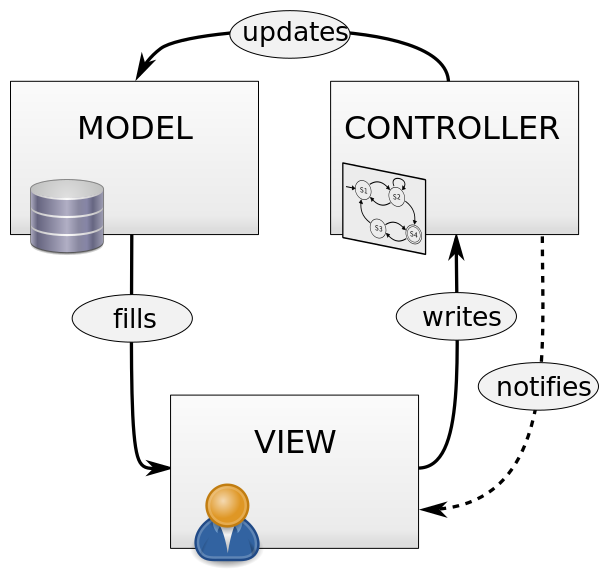
\includegraphics[width=0.6\textwidth]{img/mvc_diagram.png}
			\caption{MVC diagram \cite{MVCDiagram}}
			\label{fig:mvc_diagram}
		\end{figure}
		
	\subsection{Composer}\label{sec:composer}
	Composer je nástroj pro správu závislostí pro jazyk PHP. Umožňuje nám v~projektu deklarovat, které cizí knihovny (resp. balíčky) budou v~projektu použity. Ty poté dokáže nainstalovat nebo aktualizovat. Ve své funkcionalitě je velmi podobný jako NPM (viz sekce \ref{sec:npm}). \cite{Composer}
	
	V~tomto projektu byl použit primárně ke správě balíčků pro backendovou část.
		
\section{Úložiště dat}
Samotná data, která jsou spravována a vyměňována mezi backendem a frontendem musí být samozřejmě někde ukládána. Kromě zmíněných dat samozřejmě musí být i samotná aplikace někde uložena a veřejně dostupná. K~těmto účelům slouží právě úložiště dat – o~mnou využitých píši níže.

	\subsection{Webhosting}
	Webhosting je služba, díky které si můžeme pronajmout prostor na cizím vzdáleném serveru pro naše webové stránky. Poskytovatelé těchto služeb většinou nabízí i služby spojené s~provozem databází nebo e-mailové schránky. Hlavní výhodou této služby je fakt, že nemusíme fyzicky vlastnit žádný server a že nemusíme řešit administrativní úkony s~ním spojené (např. instalace specializovaného softwaru na serveru). \cite{Webhosting}
	
	Pro účely tohoto projektu bylo potřeba mít jak webový server pro nahrání celé aplikace, tak i databázový server pro uchovávání dat. O~mnou využitých poskytovatelích těchto služeb je psáno v~práci dále. 
	
		\subsubsection{DigitalOcean}
		DigitalOcean je americký poskytovatel cloudových služeb s~datovými centry po celém světě. Nabízí obrovské množství technologií a služeb – např. správu webového serveru, virtuální stroje či možnost zprostředkování databázového serveru. Celkově se společnost snaží především o~poskytnutí služeb, které budou uživatelsky přívětivé. \cite{DO1}\cite{DO2}
		
		Z~balíčku služeb, které DigitalOcean nabízí, byla pro tento projekt použita takzvaná \uv{App Platform} \cite{DO3}, do které lze jednoduše nahrát soubory webové aplikace a následně využívat webové služby.
		
		\subsubsection{Heroku}
		Heroku je cloudová platforma, která je využívána k~nasazení, správě a škálování moderních aplikací. V~rámci nabízených služeb se velmi podobá DigitalOceanu – nabízí tedy např. možnost využití virtuálních strojů a služby s~tím spojené nebo možnost zprostředkování nejrůznějších databázových serverů. \cite{Heroku1}\cite{Heroku2}
		
		V~rámci této implementace byla od Heroku využita služba zprostředkovávající databázové služby – konkrétně PostgreSQL server. 
		
	\subsection{Databáze}
	Databáze je organizovaná kolekce strukturovaných dat, která je v~dnešní době běžně uchovávána elektronicky. Je většinou řízena tzv. database management systémem (DBMS), který zajištuje veškerou administrativu nad daty. Data a DBMS dohromady tvoří databázový systém. Cílem moderní databáze je např. zajistit zpracování a uchovávání velkého množství dat, zabezpečení dat, dostupnost dat, možnost správy a údržby systému či škálovatelnost. Za předchůdce databáze lze považovat např. kartotéku u~lékaře. \cite{DBSummary}
	
	
	
	Databáze můžeme dělit podle modelu, který svou strukturou a funkcionalitou splňují. Základní modely jsou uvedeny níže: \cite{DBModel}
		
	\begin{itemize}
		\item \textbf{Hierarchický model} – data jsou uspořádána do stromové struktury, kde jsou omezena vztahem „jeden k~více“ (záznam z~vyšší úrovně lze spojit jen se záznamy nižší úrovně), jsou identifikovány tzv. ukazatelem (ten ukazuje na místo v~databázi, kde jsou data uložena). \cite{HierarchDB}
		\item \textbf{Síťový model} – data jsou uspořádána jako uzly rovinného grafu, jsou identifikovány tzv. ukazatelem; oproti hierarchickému modelu lze spojovat záznamy libovolně. \cite{SitDB} 
		\item \textbf{Relační model} – data jsou uspořádána v~tabulkách do relací (tj. spojení dat, která obsahují nějaký společný atribut), jsou identifikovány primárním klíčem. \cite{RelacDB}
		\item \textbf{Objektově orientovaný model} – data jsou reprezentována jako objekty, které vychází z~objektově-orientovaného programování. \cite{OOPDB}
	\end{itemize}
	
	K~zajištění možnosti ovládání databáze musí být také zajištěn způsob, jakým lze s~databází komunikovat. K~těmto účelům vznikly tzv. dotazovací jazyky, které právě slouží ke komunikaci uživatele s~příslušným programem \cite{DotazJazyk} - zde databázovým systémem. Mezi nejpoužívanější jazyky tohoto druhu patří jazyk SQL, který je primárně používán s~relačními databázemi \cite{SQL}.
	
	Dalším důležitým faktorem je spolehlivost databáze. K~tomuto účelu slouží tzv. zásady ACID - ty garantují, že data po jednotlivých úkonech nebo transakcích (zjednodušeně skupiny úkonů \cite{Transakce}) - např. aktualizace dat - budou přesná a konzistentní i při selhání systému. Zkratku ACID lze rozdělit na tyto části:
	
	\begin{itemize}
		\item \textbf{Atomicity} (v~překladu Atomicita) - buď se transakce provede celá, nebo se data nijak nezmění
		\item \textbf{Consistency} (v~překladu Konzistence) - data musí být validní a konzistentní - tzn. že musí splňovat požadavky databázového systému např. platný typ vstupní hodnoty pro určitý atribut
		\item \textbf{Isolation} (v~překladu Izolace) - všechny transakce musí na sobě být nezávislé a nesmí se nějak ovlivňovat
		\item \textbf{Durability} (v~překladu Odolnost) - po provedení transakce musí být data permanentně uložena v~databázi
		\cite{ACID}
	\end{itemize}
	
	V~projektu byla využita relační databáze PostgreSQL, která je popsána dále.
	
		\subsubsection{PostgreSQL}
		PostgreSQL je open-source objektově-relační databáze (spojení relačního a objektově orientovaného modelu) splňující ACID zásady. Je rozšířená a oblíbená kvůli její architektuře, výkonnosti, spolehlivosti, datové integritě, rozšířitelnosti, škálovatelnosti a velkému množství funkcí. Využívá jazyk SQL, který rozšiřuje o~další funkce a syntaxi. \cite{PostgreSQL}
